\documentclass[tikz,border=8pt]{standalone}
\usepackage{pgfplots}
\pgfplotsset{compat=1.18}
\begin{document}
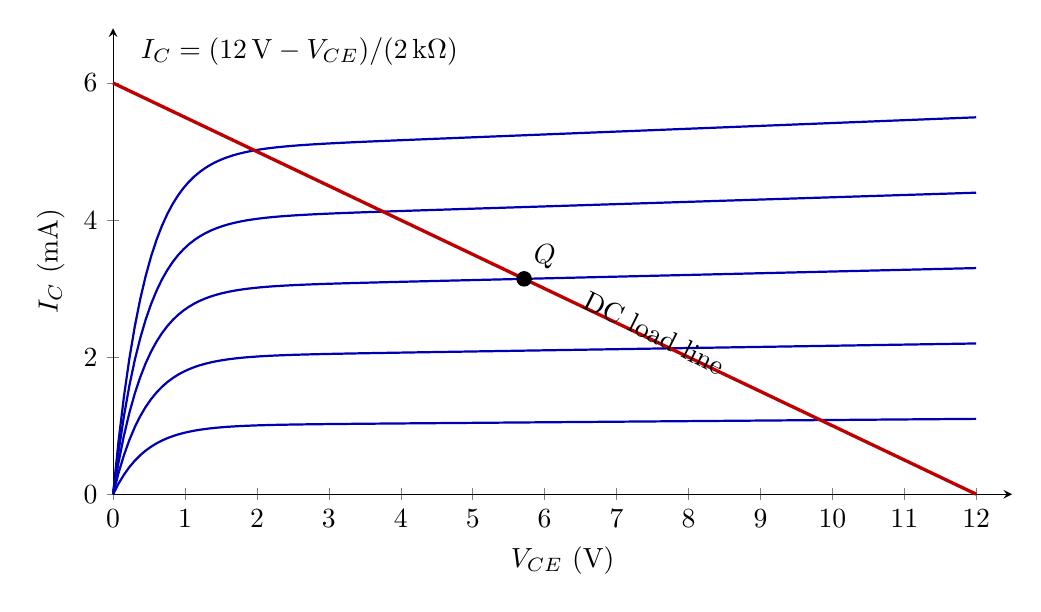
\begin{tikzpicture}
\begin{axis}[width=13cm,height=7.5cm,xmin=0,xmax=12.5,ymin=0,ymax=6.8,
 axis lines=left,xlabel={$V_{CE}$ (V)},ylabel={$I_C$ (mA)},
 legend style={at={(0.5,-0.18)},anchor=north,legend columns=3,draw=none},clip=false]
\foreach \b in {1,2,3,4,5}{\addplot[blue!70!black,thick,domain=0:12,samples=160]{\b*(1-exp(-x/0.45))*(1+x/120)};}
\addplot[red!75!black,very thick,domain=0:12]{6-x/2};
\addplot[only marks,mark=*,mark size=2.6pt,black] coordinates {(5.714304,3.142848)};
\node[anchor=south west] at (axis cs:5.714304,3.142848) {$Q$};
\node[anchor=south west] at (axis cs:0.25,6.12) {$I_C=(12\,\mathrm V-V_{CE})/(2\,\mathrm{k\Omega})$};
\node[rotate=-26.5,anchor=south] at (axis cs:7.4,2.1) {DC load line};
\end{axis}
\end{tikzpicture}
\end{document}
